\subsection{Euclidean distance}
\label{section:Euclidean}

\begin{figure}[t]
    \centering
    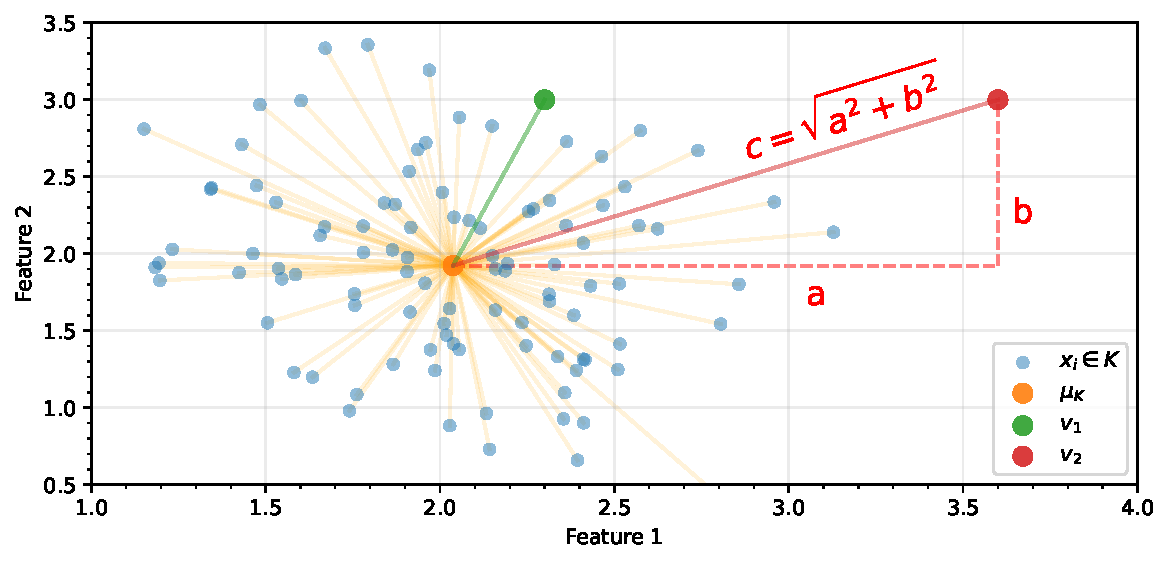
\includegraphics[width=\textwidth]{images/measures/euclidean-distance.pdf}
    \caption{Idea of the Euclidean distance applied as an outlierness measure. \\
             The location $\mu_T$ of the cluster $T$ center is identified and then involved
             in calculation of~the~outlierness scores (Minkowski metric of order $2$) for elements $v_1$ and $v_2$.}
    \label{fig:ed-idea}
\end{figure}

The Euclidean distance is an intuitive baseline method for quantifying the similarity based on the distance. In this approach, the data cluster $T$ is represented by a middle point $\mu_{T}$, calculated as an average of all ($n_{T} = \abs{T}$) feature vectors $x_i$, $x_i \in T$,
\begin{equation}
    \mu_{T} = \frac{1}{n_{T}} \cdot \sum_{i=1}^{n_{T}} x_i
    ~.
    \label{eq:mu_T}
\end{equation}

The outlierness score for a given vector $v$ against the data cluster $T$ is then calculated as the Minkowski distance of order $2$ in $\mathbb{R}^d$ space between the $v$ and point $\mu_{T}$ location,
\begin{equation}
    ED(v, T) = \norm{\vv{v - \mu_{T}}}
    .
    \label{eq:ed}
\end{equation}

Figure \ref{fig:ed-idea} presents the idea of leveraging such simple method for outlier detection. Any element $v$ that is further than acceptable threshold can be marked as outlier ($v_2$), wheres object at typical distance is considered as in-distribution ($v_1$). This approach is suitable as long as the data are evenly distributed on all axes in $\mathbb{R}^d$ space and also not affected by any correlation. Otherwise the risk of spurious ID/OOD label assignment increases, especially in high-dimensional feature spaces.

During the research the implementation from the SciPy library \cite{SciPy-NMeth} was utilized.
